\documentclass[11pt,a4paper]{report}
\usepackage[portuguese]{babel}
\usepackage[utf8]{inputenc}
\usepackage[T1]{fontenc}
\usepackage{glossaries}
\usepackage{graphicx}
\usepackage{hyperref}
\usepackage{wrapfig}
\usepackage{float}
\usepackage{natbib}
\newcommand{\HRule}{\rule{\linewidth}{0.5mm}}

\title{\textbf{Artesanato de Aveiro} \\ 
\large{Sistemas Distribuídos\\ Problema Obrigatório 2}\\
\normalsize{Universidade de Aveiro}
}
\author{\normalsize{Docente - António Rui Borges}
\\
\\ Prática 4
\\ Grupo 5
\\
\\
\normalsize{Diogo Silva 60337} \\
\normalsize{Tânia Alves 60340} }

\begin{document}
\maketitle
\tableofcontents

\chapter{Descrição das Mensagens}

\subsubsection{COLLECTING\_MATERIALS}
Argumentos:
\begin{enumerate}
\itemsep-0.4em 
\item Identificador do craftsman
\end{enumerate}
Possiveis respostas: 
\begin{enumerate}
\itemsep-0.4em 
\item POSITIVE, no caso de ainda haver materiais para fazer uma peça
\item NEGATIVE, quando já não houver materiais necessários
\end{enumerate}

\subsubsection{PRIME\_MATERIALS\_NEEDED}
Argumentos:
\begin{enumerate}
\itemsep-0.4em 
\item Identificador do craftsman
\end{enumerate}
Possiveis respostas: 
\begin{enumerate}
\itemsep-0.4em 
\item ACK, para informar que a mensagem foi recebida com sucesso.
\end{enumerate}

\subsubsection{BACK\_TO\_WORK}
Argumentos:
\begin{enumerate}
\itemsep-0.4em 
\item Identificador do craftsman
\end{enumerate}
Possiveis respostas: 
\begin{enumerate}
\itemsep-0.4em 
\item ACK, para informar que a mensagem foi recebida com sucesso.
\end{enumerate}

\subsubsection{PREPARE\_TO\_PRODUCE}
Argumentos:
\begin{enumerate}
\itemsep-0.4em 
\item Identificador do craftsman
\end{enumerate}
Possiveis respostas: 
\begin{enumerate}
\itemsep-0.4em 
\item ACK, para informar que a mensagem foi recebida com sucesso.
\end{enumerate}

\subsubsection{GO\_TO\_STORE}
Argumentos:
\begin{enumerate}
\itemsep-0.4em 
\item Identificador do craftsman
\end{enumerate}
Possiveis respostas: 
\begin{enumerate}
\itemsep-0.4em 
\item ACK com o número de produtos armazenados no Workshop.
\end{enumerate}

\subsubsection{BATCH\_READY\_FOR\_TRANSFER}
Argumentos:
\begin{enumerate}
\itemsep-0.4em 
\item Identificador do craftsman
\end{enumerate}
Possiveis respostas: 
\begin{enumerate}
\itemsep-0.4em 
\item ACK, para informar que a mensagem foi recebida.
\end{enumerate}

\subsubsection{GO\_SHOPPING}
Argumentos:
\begin{enumerate}
    \itemsep-0.4em
    \item Identificador do cliente
\end{enumerate}
Possiveis respostas:
\begin{enumerate}
    \itemsep-0.4em
    \item ACK, para informar que a mensagem foi recebida com sucesso.
\end{enumerate}

\subsubsection{IS\_DOOR\_OPEN}
Sem argumentos.
Possiveis respostas:
\begin{enumerate}
    \itemsep-0.4em
    \item POSITIVE, caso a porta da loja esteja aberta
    \item NEGATIVE, case a porta da loja esteja fechada
\end{enumerate}

\subsubsection{ENTER\_SHOP}
Argumentos:
\begin{enumerate}
    \itemsep-0.4em
    \item Identificador do cliente
\end{enumerate}
Possiveis respostas:
\begin{enumerate}
    \itemsep-0.4em
    \item ACK, para informar que a mensagem foi recebida com sucesso.
\end{enumerate}

\subsubsection{PERUSING\_AROUND}
Sem argumentos.
Possiveis respostas:
\begin{enumerate}
    \itemsep-0.4em
    \item ACK, para informar que a mensagem foi recebida com sucesso.
\end{enumerate}

\subsubsection{I\_WANT\_THIS}
Argumentos:
\begin{enumerate}
    \itemsep-0.4em
    \item Identificador do cliente
    \item Número de produtos que o cliente pretende comprar
\end{enumerate}
Possiveis respostas:
\begin{enumerate}
    \itemsep-0.4em
    \item ACK, para informar que a mensagem foi recebida com sucesso.
\end{enumerate}

\subsubsection{EXIT\_SHOP}
Argumentos:
\begin{enumerate}
    \itemsep-0.4em
    \item Identificador do cliente
\end{enumerate}
Possiveis respostas:
\begin{enumerate}
    \itemsep-0.4em
    \item ACK, para informar que a mensagem foi recebida com sucesso.
\end{enumerate}

\subsubsection{TRY\_AGAIN\_LATER}
Argumentos:
\begin{enumerate}
    \itemsep-0.4em
    \item Identificador do cliente
\end{enumerate}
Possiveis respostas:
\begin{enumerate}
    \itemsep-0.4em
    \item ACK, para informar que a mensagem foi recebida com sucesso.
\end{enumerate}

\subsubsection{PREPARE\_TO\_WORK}
Sem argumentos.
Possiveis respostas:
\begin{enumerate}
    \itemsep-0.4em
    \item ACK, para informar que a mensagem foi recebida com sucesso.
\end{enumerate}

\subsubsection{APPRAISE\_SIT}
Sem argumentos.
Possiveis respostas:
\begin{enumerate}
    \itemsep-0.4em
    \item ACK, para informar que a mensagem foi recebida com sucesso.
\end{enumerate}

\subsubsection{ADDRESS\_A\_CUSTOMER}
Sem argumentos.
Possiveis respostas:
\begin{enumerate}
    \itemsep-0.4em
    \item ACK, para informar que a mensagem foi recebida com sucesso.
\end{enumerate}

\subsubsection{SAY\_GOODBYE\_TO\_CUSTOMER}
Argumentos:
\begin{enumerate}
    \itemsep-0.4em
    \item Identificador do cliente
\end{enumerate}
Possiveis respostas:
\begin{enumerate}
    \itemsep-0.4em
    \item ACK, para informar que a mensagem foi recebida com sucesso.
\end{enumerate}

\subsubsection{CLOSE\_THE\_DOOR}
Sem argumentos.
Possiveis respostas:
\begin{enumerate}
    \itemsep-0.4em
    \item ACK, para informar que a mensagem foi recebida com sucesso.
\end{enumerate}

\subsubsection{CUSTOMERS\_IN\_THE\_SHOP}
Sem argumentos.
Possiveis respostas:
\begin{enumerate}
    \itemsep-0.4em
    \item POSITIVE, caso haja clientes dentro da loja
    \item NEGATIVE, se a loja já não tiver clientes lá dentro
\end{enumerate}

\subsubsection{PREPARE\_TO\_LEAVE}
Sem argumentos.
Possiveis respostas:
\begin{enumerate}
    \itemsep-0.4em
    \item ACK, para informar que a mensagem foi recebida com sucesso.
\end{enumerate}


\subsubsection{GO\_TO\_WORKSHOP}
Sem argumentos.
Possiveis respostas:
\begin{enumerate}
    \itemsep-0.4em
    \item ACK, para informar que a mensagem foi recebida com sucesso.
\end{enumerate}

\subsubsection{RETURN\_TO\_SHOP} 
Argumentos:
\begin{enumerate}
    \itemsep-0.4em
    \item Número de produtos que a dona traz consigo
\end{enumerate}
Possiveis respostas:
\begin{enumerate}
    \itemsep-0.4em
    \item ACK, para informar que a mensagem foi recebida com sucesso.
\end{enumerate}

\subsubsection{VISIT\_SUPPLIERS}
Sem argumentos.
Possiveis respostas:
\begin{enumerate}
    \itemsep-0.4em
    \item ACK, para informar que a mensagem foi recebida com sucesso.
\end{enumerate}

\subsubsection{REPLENISH\_STOCK}
Argumentos:
\begin{enumerate}
    \itemsep-0.4em
    \item Número de matérias primas
\end{enumerate}
Possiveis respostas:
\begin{enumerate}
    \itemsep-0.4em
    \item ACK, para informar que a mensagem foi recebida com sucesso.
\end{enumerate}

\subsubsection{RESET\_REQ\_PMATERIALS}
Sem argumentos.
Possiveis respostas:
\begin{enumerate}
    \itemsep-0.4em
    \item ACK, para informar que a mensagem foi recebida com sucesso.
\end{enumerate}

\subsubsection{RESET\_REQ\_PRODUCTS}
Sem argumentos.
Possiveis respostas:
\begin{enumerate}
    \itemsep-0.4em
    \item ACK, para informar que a mensagem foi recebida com sucesso.
\end{enumerate}

\subsubsection{INIT\_WRITE}
Argumentos:
\begin{enumerate}
    \itemsep-0.4em
    \item Nome do ficheiro de logging (se for null, é gerado um novo baseado na data e hora da simulação)
\end{enumerate}
Possiveis respostas:
\begin{enumerate}
    \itemsep-0.4em
    \item ACK, para informar que a mensagem foi recebida com sucesso.
\end{enumerate}

\subsubsection{END\_WRITE}
Sem argumentos.
Possiveis respostas:
\begin{enumerate}
    \itemsep-0.4em
    \item ACK, para informar que a mensagem foi recebida com sucesso.
\end{enumerate}

\subsubsection{END\_OPER\_CUSTOMER}
Sem argumentos.
Possiveis respostas:
\begin{enumerate}
    \itemsep-0.4em
    \item POSITIVE se o cliente da loja poder terminar a sua execução
    \item NEGATIVE se o cliente ainda não poder terminar a sua execução
\end{enumerate}

\subsubsection{END\_OPER\_CRAFTSMAN}
Sem argumentos.
Possiveis respostas:
\begin{enumerate}
    \itemsep-0.4em
    \item NEGATIVE se o artesão ainda não poder terminar a sua execução
    \item POSITIVE, com uma flag a false, se o artesão já poder terminar a sua execução sem ser necessário mais nenhuma operação
    \item POSITIVE, com uma flag a true, se o artesão já poder terminar a sua execução, mas tiver de fazer um pedido de transferência de produtos antes
\end{enumerate}

\subsubsection{END\_OPER\_ENTREPRENEUR}
Sem argumentos.
Possiveis respostas:
\begin{enumerate}
    \itemsep-0.4em
    \item POSTIVE, se a dona poder terminar a sua execução
    \item NEGATIVE, se a dona não poder terminar a sua execução
\end{enumerate}

\subsubsection{UPDATE\_REQ\_PMATERIALS}
Argumentos:
\begin{enumerate}
    \itemsep-0.4em
    \item Flag que indica se há um pedido de matérias primas ou não
\end{enumerate}
Possiveis respostas:
\begin{enumerate}
    \itemsep-0.4em
    \item ACK, para informar que a mensagem foi recebida com sucesso.
\end{enumerate}

\subsubsection{UPDATE\_REQ\_PRODUCTS}
Argumentos:
\begin{enumerate}
    \itemsep-0.4em
    \item Flag que indica se há um pedido de transferência de produtos ou não
\end{enumerate}
Possiveis respostas:
\begin{enumerate}
    \itemsep-0.4em
    \item ACK, para informar que a mensagem foi recebida com sucesso.
\end{enumerate}

\subsubsection{WRITE\_ENTR\_STATE}
Argumentos:
\begin{enumerate}
    \itemsep-0.4em
    \item Estado da dona
\end{enumerate}
Possiveis respostas:
\begin{enumerate}
    \itemsep-0.4em
    \item ACK, para informar que a mensagem foi recebida com sucesso.
\end{enumerate}

\subsubsection{WRITE\_CRAFT\_STATE}
Argumentos:
\begin{enumerate}
    \itemsep-0.4em
    \item Identificador do artesão
    \item Estado do artesão
\end{enumerate}
Possiveis respostas:
\begin{enumerate}
    \itemsep-0.4em
    \item ACK, para informar que a mensagem foi recebida com sucesso.
\end{enumerate}

\subsubsection{WRITE\_CUST\_STATE}
Argumentos:
\begin{enumerate}
    \itemsep-0.4em
    \item Identificador do cliente
    \item Estado do cliente
\end{enumerate}
Possiveis respostas:
\begin{enumerate}
    \itemsep-0.4em
    \item ACK, para informar que a mensagem foi recebida com sucesso.
\end{enumerate}

\subsubsection{WRITE\_SHOP}
Argumentos:
\begin{enumerate}
    \itemsep-0.4em
    \item Estado da loja
    \item Número de clientes dentro da loja
    \item Número de produtos expostos na loja
    \item Flag de pedido de transferência de produtos
    \item Flag de pedido de matérias primas
\end{enumerate}
Possiveis respostas:
\begin{enumerate}
    \itemsep-0.4em
    \item ACK, para informar que a mensagem foi recebida com sucesso.
\end{enumerate}

\subsubsection{WRITE\_SHOP\_ENTR\_STATE}
Argumentos:
\begin{enumerate}
    \itemsep-0.4em
    \item Estado da dona
    \item Estado da loja
    \item Número de clientes dentro da loja
    \item Número de produtos expostos na loja
    \item Flag de pedido de transferência de produtos
    \item Flag de pedido de matérias primas
\end{enumerate}
Possiveis respostas:
\begin{enumerate}
    \itemsep-0.4em
    \item ACK, para informar que a mensagem foi recebida com sucesso.
\end{enumerate}
    
\subsubsection{WRITE\_SHOP\_CRAFT\_STATE}
Argumentos:
\begin{enumerate}
    \itemsep-0.4em
    \item Estado da loja
    \item Número de clientes dentro da loja
    \item Número de produtos expostos na loja
    \item Estado do artesão
    \item Identificador do artesão
    \item Flag de pedido de transferência de produtos
    \item Flag de pedido de matérias primas
\end{enumerate}
Possiveis respostas:
\begin{enumerate}
    \itemsep-0.4em
    \item ACK, para informar que a mensagem foi recebida com sucesso.
\end{enumerate}

\subsubsection{WRITE\_SHOP\_CUST\_STATE}
Argumentos:
\begin{enumerate}
    \itemsep-0.4em
    \item Estado da loja
    \item Número de clientes dentro da loja
    \item Número de produtos expostos na loja
    \item Flag de pedido de transferência de produtos
    \item Flag de pedido de matérias primas
    \item Estado do cliente
    \item Identificador do cliente
    \item Número de produtos comprados pelo cliente até ao momento
\end{enumerate}
Possiveis respostas:
\begin{enumerate}
    \itemsep-0.4em
    \item ACK, para informar que a mensagem foi recebida com sucesso.
\end{enumerate}

\subsubsection{WRITE\_WSHOP}
Argumentos:
\begin{enumerate}
    \itemsep-0.4em
    \item Número de matérias primas actual
    \item Número de produtos em armazém
    \item Número de vezes que foram entregues matérias primas
    \item Número total de matérias primas que foram entregues até ao momento
    \item Número de produtos terminados até ao momento
\end{enumerate}
Possiveis respostas:
\begin{enumerate}
    \itemsep-0.4em
    \item ACK, para informar que a mensagem foi recebida com sucesso.
\end{enumerate}

\subsubsection{WRITE\_WSHOP\_CRAFT\_STATE}
Argumentos:
\begin{enumerate}
    \itemsep-0.4em
    \item Número de matérias primas actual
    \item Número de produtos em armazém
    \item Número de vezes que foram entregues matérias primas
    \item Número total de matérias primas que foram entregues até ao momento
    \item Número de produtos terminados até ao momento
    \item Estado do artesão
    \item Identificador do artesão
    \item Flag que indica se o artesão tem mais uma peça acabada
\end{enumerate}
Possiveis respostas:
\begin{enumerate}
    \itemsep-0.4em
    \item ACK, para informar que a mensagem foi recebida com sucesso.
\end{enumerate}

\subsubsection{WRITE\_WSHOP\_ENTR\_STATE}
Argumentos:
\begin{enumerate}
    \itemsep-0.4em
    \item Number of products stored
    \item Number of times prime materials were fetched
    \item Number of total prime materials supplied
    \item Number of finished products
    \item Entrepreneur state
\end{enumerate}
Possiveis respostas:
\begin{enumerate}
    \itemsep-0.4em
    \item ACK, para informar que a mensagem foi recebida com sucesso.
\end{enumerate}

\subsubsection{TERMINATE}
Sem argumentos.
Possiveis respostas: 
\begin{enumerate}
\itemsep-0.4em 
\item ACK, para informar que a mensagem foi recebida com sucesso.
\end{enumerate}

\subsubsection{TERMINATED}
Sem argumentos.
Possiveis respostas: 
\begin{enumerate}
\itemsep-0.4em 
\item ACK, para informar que a mensagem foi recebida com sucesso.
\end{enumerate}

\chapter{Diagrama de Interacção}

Foi considerado o esquema introduzido durante as aulas para a representação do diagrama de interecção.

\begin{figure}[h]
    \centering
    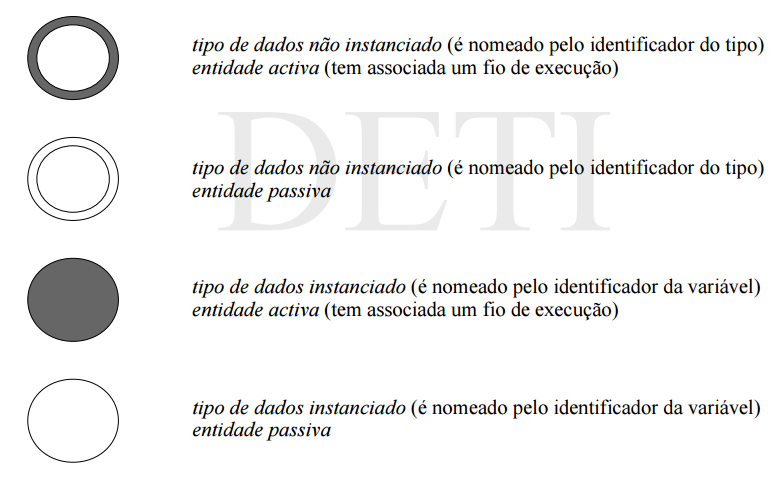
\includegraphics[width=1\textwidth]{images/schema.png}
    \caption{Esquema utilizado para representar o diagrama de interecção. Retirado a partir do moodle da unidade curricular de Sistemas Distribuídos}
    \label{fig:awesome_image}
\end{figure}
\newpage
\section{Servidores}

\subsection{Logging}
\begin{figure}[h]
    \centering
    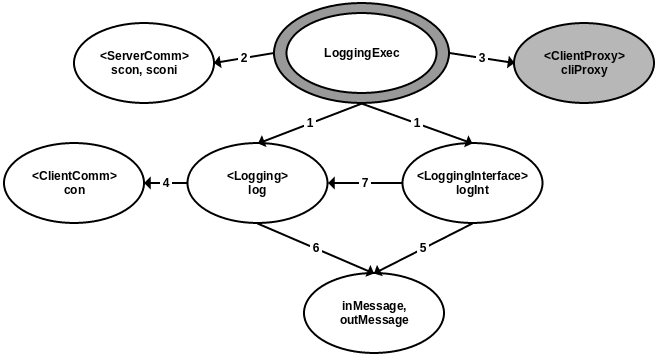
\includegraphics[width=0.9\textwidth]{images/logging.png}
    \caption{Diagrama de Interacção do servidor Logging}
    \label{fig:awesome_image}
\end{figure}

\begin{enumerate}
\itemsep-0.4em 
%% 1. 
\item instantiate
\item instantiate, start, accept
\item instantiate, start
\item instantiate, readObject, writeObject
\item instantiate, getType, isRequestPrimeMaterials, isRequestFetchProducts, getEntrState, getCraftState, getCustState, getId, getShopState, getnCustomerIn, getnGoodsInDisplay, getnBoughtGoods, getnCurrentPrimeMaterials, getnProductsStored, getnTimesPrimeMaterialsFetched, getnTotalPrimeMaterialsSupplied, getnFinishedProducts, isFinishedProduct
\item instantiate, getType
\item WriteWorkshopAndEntrepreneurStat, WriteWorkshopAndCraftsmanStat, WriteWorkshop, WriteShopAndCustomerStat, WriteShopAndCraftsmanStat, WriteShopAndEntrepreneurStat, WriteShop, UpdateCustomerState, UpdateEntreperneurState, UpdateFetchProductsRequest, UpdatePrimeMaterialsRequest, endOpEntrep, endOperCraft, endOpCustomer, clientsTerminated, terminateServers
\end{enumerate}

\newpage
\subsection{Shop}

\begin{figure}[h]
    \centering
    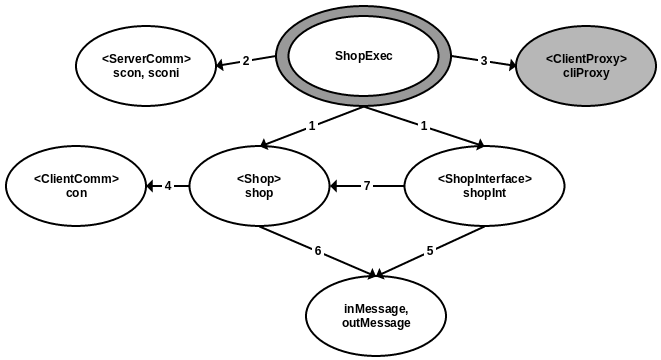
\includegraphics[width=0.9\textwidth]{images/shop.png}
    \caption{Diagrama de Interacção do servidor Shop}
    \label{fig:awesome_image}
\end{figure}

\begin{enumerate}
\itemsep-0.4em 
%% 1. 
\item instantiate
\item instantiate, start, accept
\item instantiate, start
\item instantiate, readObject, writeObject
\item instantiate, getType, getId, getnProducts
\item instantiate, getType
\item goShopping, isDoorOpen, enterShop, exitShop, iWantThis, tryAgainLater, prepareToWork, appraiseSit, addressACustomer, sayGoodByeToCustomer, closeTheDoor, customersInTheShop, prepareToLeave, returnToShop, primeMaterialsNeeded, batchReadyForTransfer, resetRequestPrimeMaterials, resetRequestProducts
\end{enumerate}
\newpage
\subsection{Warehouse}

\begin{figure}[h]
    \centering
    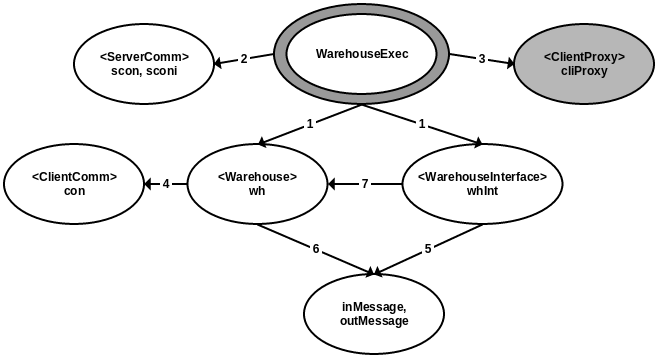
\includegraphics[width=0.9\textwidth]{images/warehouse.png}
    \caption{Diagrama de Interacção do servidor Warehouse}
    \label{fig:awesome_image}
\end{figure}

\begin{enumerate}
\itemsep-0.4em 
%% 1. 
\item instantiate
\item instantiate, start, accept
\item instantiate, start
\item instantiate, readObject, writeObject
\item instantiate, getType
\item instantiate, getType
\item visitSuppliers
\end{enumerate}
\newpage
\subsection{Workshop}

\begin{figure}[h]
    \centering
    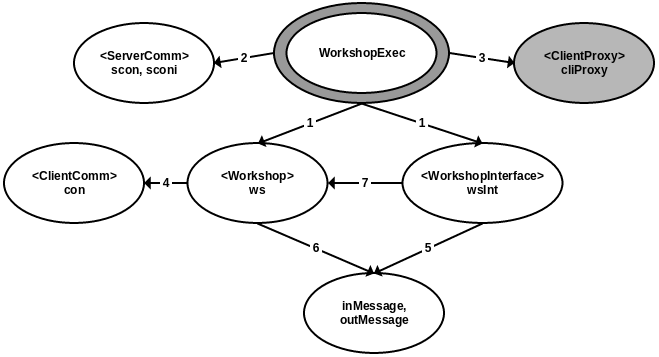
\includegraphics[width=0.9\textwidth]{images/workshop.png}
    \caption{Diagrama de Interacção do servidor Workshop}
    \label{fig:awesome_image}
\end{figure}

\begin{enumerate}
\itemsep-0.4em 
%% 1. 
\item instantiate
\item instantiate, start, accept
\item instantiate, start
\item instantiate, readObject, writeObject
\item instantiate, getType, getnMaterials, getId
\item instantiate, getType
\item goToWorkshop, replenishStock, collectingMaterials, goToStore, backToWork, prepareToProduce
\end{enumerate}
\newpage
\section{Clientes}

\subsection{Entrepreneur}

\begin{figure}[h]
    \centering
    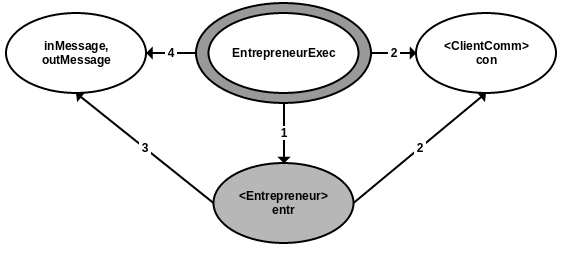
\includegraphics[width=0.9\textwidth]{images/entrepreneur.png}
    \caption{Diagrama de Interacção do cliente Entrepreneur}
    \label{fig:awesome_image}
\end{figure}

\begin{enumerate}
\itemsep-0.4em 
%% 1. 
\item instantiate, start, join
\item instantiate, writeObject, readObject
\item instantiate, getType, getEntrState, getNextTask, getReturnEntr
\item instantiate, getType
\end{enumerate}

\subsection{Craftsman}

\begin{figure}[h]
    \centering
    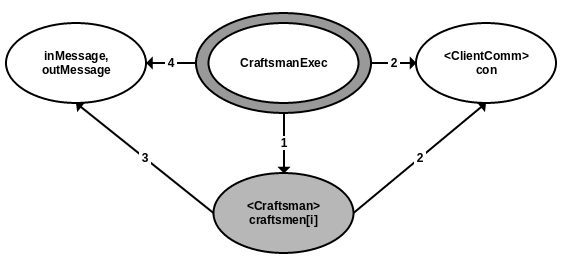
\includegraphics[width=0.9\textwidth]{images/craftsman.png}
    \caption{Diagrama de Interacção do cliente Craftsman}
    \label{fig:awesome_image}
\end{figure}

\begin{enumerate}
\itemsep-0.4em 
%% 1. 
\item instantiate, start, join
\item instantiate, writeObject, readObject
\item instantiate, getType, getCraftState, getnProductsStored, isRequestFetchProducts
\item instantiate, getType
\end{enumerate}

\subsection{Customer}

\begin{figure}[h]
    \centering
    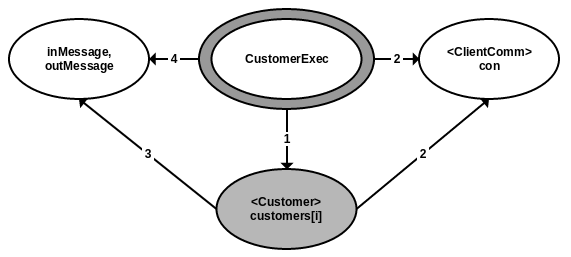
\includegraphics[width=0.9\textwidth]{images/customer.png}
    \caption{Diagrama de Interacção do cliente Customer}
    \label{fig:awesome_image}
\end{figure}

\begin{enumerate}
\itemsep-0.4em 
%% 1. 
\item instantiate, start, join
\item instantiate, writeObject, readObject
\item instantiate, getType, getCustState, getnProducts
\item instantiate, getType
\end{enumerate}


\end{document}


